\documentclass[tikz,border=8pt]{standalone}

\usepackage{amsmath}
\usetikzlibrary{arrows.meta,positioning,calc}

\begin{document}
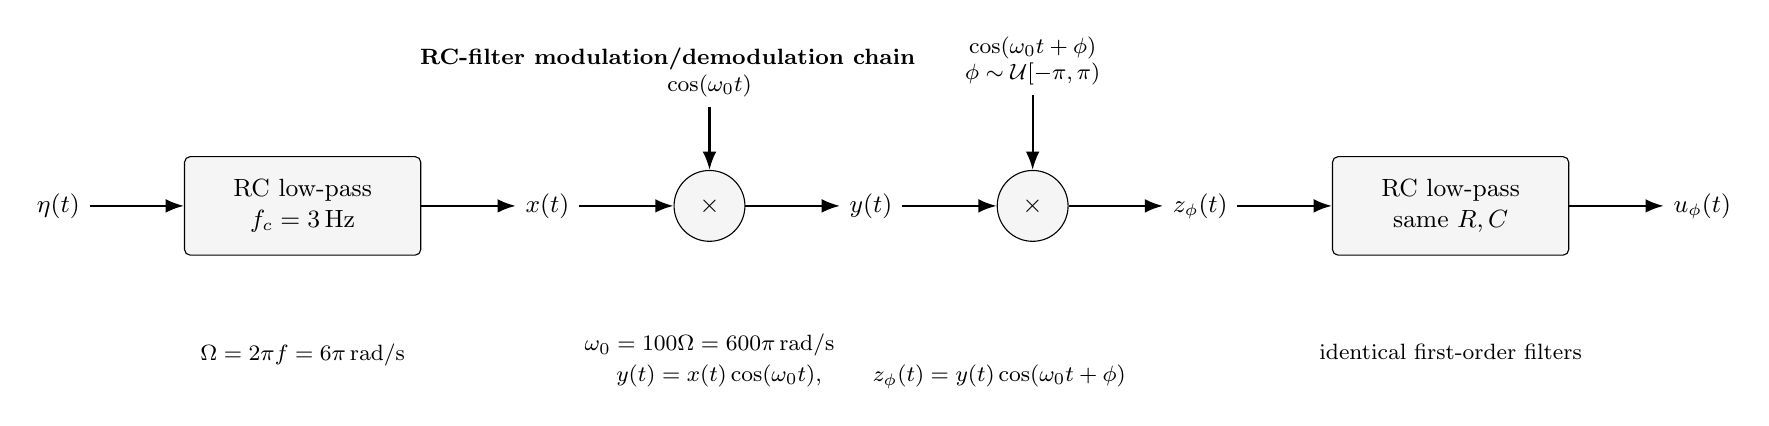
\begin{tikzpicture}[
  font=\small,
  >=Latex,
  node distance=1.7cm and 1.2cm,
  line/.style={-Latex, thick},
  block/.style={
    draw,
    rounded corners=2pt,
    minimum width=3.0cm,
    minimum height=1.25cm,
    align=center,
    fill=gray!8
  },
  mixer/.style={
    draw,
    circle,
    minimum size=9mm,
    inner sep=0pt,
    fill=gray!8
  },
  note/.style={
    align=center,
    font=\footnotesize
  }
]

\node (eta) {$\eta(t)$};

\node[block, right=of eta] (lpf1) {RC low-pass\\$f_c = 3\,\mathrm{Hz}$};
\node[right=of lpf1] (x) {$x(t)$};

\node[mixer, right=of x] (mix1) {$\times$};
\node[right=of mix1] (y) {$y(t)$};

\node[mixer, right=of y] (mix2) {$\times$};
\node[right=of mix2] (z) {$z_\phi(t)$};

\node[block, right=of z] (lpf2) {RC low-pass\\same $R,C$};
\node[right=of lpf2] (u) {$u_\phi(t)$};

\draw[line] (eta) -- (lpf1);
\draw[line] (lpf1) -- (x);
\draw[line] (x) -- (mix1);
\draw[line] (mix1) -- (y);
\draw[line] (y) -- (mix2);
\draw[line] (mix2) -- (z);
\draw[line] (z) -- (lpf2);
\draw[line] (lpf2) -- (u);

\node[note, above=0.8cm of mix1] (txnote) {$\cos(\omega_0 t)$};
\draw[line] (txnote) -- (mix1);

\node[note, above=0.95cm of mix2] (rxnote) {$\cos(\omega_0 t + \phi)$\\$\phi \sim \mathcal{U}[-\pi,\pi)$};
\draw[line] (rxnote) -- (mix2);

\node[note, below=1.0cm of lpf1] {$\Omega = 2\pi f = 6\pi\,\mathrm{rad/s}$};
\node[note, below=1.05cm of mix1] {$\omega_0 = 100\Omega = 600\pi\,\mathrm{rad/s}$};
\node[note, below=1.0cm of lpf2] {identical first-order filters};

\node[note, above=1.6cm of $(lpf1)!0.5!(mix2)$] (title)
  {\textbf{RC-filter modulation/demodulation chain}};

\node[note, below=1.9cm of $(mix1)!0.5!(mix2)$] (eqn)
  {$y(t)=x(t)\cos(\omega_0 t), \qquad z_\phi(t)=y(t)\cos(\omega_0 t+\phi)$};

\end{tikzpicture}
\end{document}
